\documentclass[12pt]{ctexart} % 使用 ctexart 文档类支持中文

\usepackage{fancyhdr} % 奇特的 header
\usepackage{xcolor} % 更多颜色

\usepackage[utf8]{inputenc} % 支持 UTF8 字符,在 UTF8 engine 中无需此行
\usepackage{xeCJK} % 支持中文排版,已经包含在 ctexart 中
\usepackage{fontspec} % 字体设置
\usepackage{geometry} % 页面布局
\usepackage{titlesec} % 自定义标题样式
\usepackage{setspace} % 设置行距
\usepackage{microtype} % 更多的微调
\usepackage{tabularx} % 表格支持
\usepackage{booktabs} 
\usepackage{float} % Add the float package,支持图片位置固定

\usepackage[colorlinks,linkcolor=black,urlcolor=black]{hyperref} % 超链接支持

\usepackage{tocloft} % 自定义目录样式

\usepackage{graphicx} % 图片设置
\graphicspath{ {./images/} }

% 设置页面布局
\geometry{a4paper, margin=1in}

% 设置行距为 1.25 倍
\setstretch{1.25}

% 设置中文字体
\setCJKmainfont{SimSun}[BoldFont={Microsoft YaHei Bold}] % 设置正文为宋体

\setCJKsansfont{Microsoft YaHei}[BoldFont={Microsoft YaHei Bold}] % 标题等无衬线字体为黑体

% 设置英文字体
\setmainfont{Times New Roman}



% 配置页眉和页脚
\pagestyle{fancy}
\fancyhf{}

\renewcommand{\headrulewidth}{0pt}

\setlength{\headheight}{25.60938pt} % Set the headheight to the required value
\addtolength{\topmargin}{-13.60938pt} % Adjust the topmargin to compensate

% 定义颜色
\definecolor{myred}{RGB}{244, 67, 54} % 蓝色

% 左侧页眉设置, 页码在页眉外侧
\fancyhead[L]{%
  \colorbox{myred}{%
    \parbox[t]{1cm}{%
      \textcolor{white}{\thepage}%
    }%
  }%
  \hspace{0.5cm}
  测试报告
}

% \fancyhead[L]{\leftmark} % 左页显示章节名

% 页眉横线设置
\renewcommand{\headrulewidth}{0.5pt}
\renewcommand{\headrule}{%
  \hbox to\headwidth{%
    \color{black}\leaders\hrule height \headrulewidth\hfill%
  }%
}

% 页脚页数设置
\renewcommand{\footrulewidth}{0pt}
\fancyfoot[C]{\thepage}

% 设置目录样式
\renewcommand{\cftsecfont}{\bfseries} % 目录中章节标题加粗

\titleformat{\section}
  {\normalfont\Large\bfseries} % 移除 \centering
  {\thesection}{1em}{}


% 超链接设置
\hypersetup{
  colorlinks=true,
  linkcolor=black,
  filecolor=magenta,      
  urlcolor=magenta,
}

\begin{document}

\begin{titlepage}
  \centering % 居中对齐
  % \vspace*{1cm} % 从顶部添加一些垂直间距
  
\includegraphics[width=0.6\textwidth]{zjutitle.jpg} % 插入图片
  
  \vspace{2cm} % 添加垂直间距
  
  {\fontsize{36}{48}\selectfont\CJKfontspec{Microsoft YaHei} 测试报告} % 标题
  
  \vspace{2cm} % 添加垂直间距
  
  
\includegraphics[width=0.4\textwidth]{zjulogo.jpg} % 插入图片
  
  \vspace{2cm}
  
  {\Huge\CJKfontspec{Microsoft YaHei} 项目主题: \underline{H5游戏分享平台}} % 项目主题 with underline
  
  \vspace{1cm}

  {\Large\CJKfontspec{Microsoft YaHei} 第 1 小组: \underline{XXX}} % 作者
  
  \vspace{1cm} % 添加垂直间距
  
  {\Large\CJKfontspec{Microsoft YaHei} \today} % 日期

\end{titlepage}

\newpage
\tableofcontents % 自动生成目录
\newpage

\section{引言}



\subsection{编写目的}

软件需求规则说明书描述了“H5 游戏分享平台”的软件功能性需求和非功能性需求。这一文档旨在对开发人员的工作有一个总体的评估,以及对测试计划文档中测试人员的工作进行评估,还有对最后产品的质量性能的评测。
\subsection{定义}

功能测试(Functional Testing):也称为行为测试(Behavioral Testing),根据产品特征、操作描述和用户方案,测试一个产品的特性和可操作行为以确定它们满足设计需求。本地化软件的功能测试,用于验证应用程序或网站对目标用户能正确工作。使用适当的平台、浏览器和测试脚本,以保证目标用户的体验将足够好,就像应用程序是专门为该市场开发的一样。

边界测试(Boundary Testing):边界测试用来探测和验证代码在处理极端的或偏门的情况时会发生什么。

压力测试(Stress Testing):软件压力测试是一种基本的质量保证行为,它是每个重要软件测试工作的一部分。软件压力测试的基本思路很简单:不是在常规条件下运行手动或自动测试,而是在计算机数量较少或系统资源匮乏的条件下运行测试。通常要进行软件压力测试的资源包括内部内存、CPU可用性、磁盘空间和网络带宽。

接口测试(Interface Communication Testing):接口测试的目的是测试接口(外部的或内部的),尤其是那些与系统相关联的外部接口。测试的重点是要检查数据的交换,传递和控制管理过程,还包括处理的次数。外部接口测试一般是作为系统测试来看待的。

边界值分析(Boundary Value Analysis, BVA):边界值分析法就是对输入或输出的边界值进行测试的一种黑盒测试方法。通常边界值分析法是作为对等价类划分法的补充,这种情况下,其测试用例来自等价类的边界。
\subsection{参考资料}

《软件设计文档国家标准》

《软件工程项目开发文档范例》

《Software Requirements edition2》Karl E. Wiegers

《软件需求》刘伟琴、刘洪涛译
\section{面向对象测试}

\subsection{系统整体架构}

  \begin{figure}[H] % 使用 figure 环境来插入图片
      \centering % 图片居中
      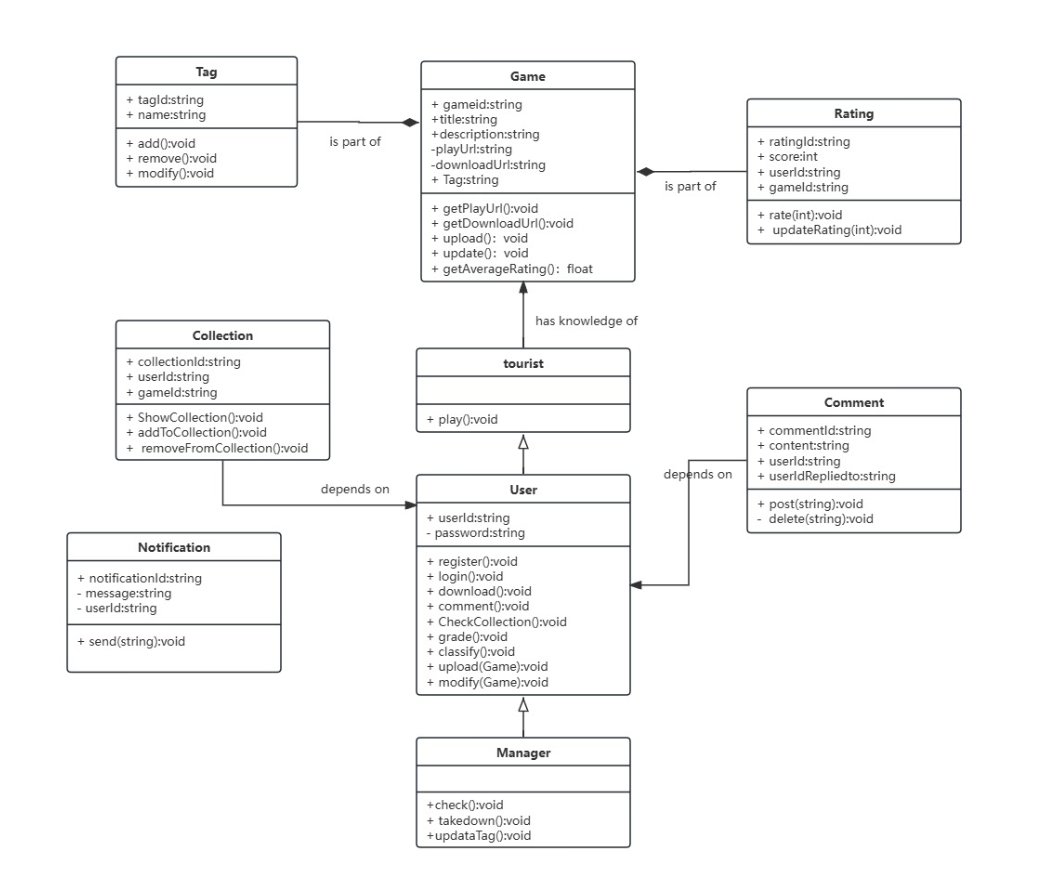
\includegraphics[width=0.8\textwidth]{./images/class.png} % 插入图片,设置宽度为页面宽度的 50%
      \caption{总体架构图} % 添加标题
  \end{figure}

在这个图中,可以看出我们使用game类,这个类是我们整个系统的核心类,所有的功能都围绕着这个类进行设计。
我们可以看到这个类需要tag类和rating类的支持,tag类是用来对游戏进行分类的,而rating类是用来对游戏进行评分的。

tourist类是实现用户在线游玩游戏的需求,它需要知道游戏全部信息。User类是需要实现登录、下载、打分、分类、上传游戏和修改游戏等功能。
而管理者可以检查游戏,下架游戏,更新标签的功能。接下来,我们将结合具体类的功能进行具体的测试。

\subsection{单元测试}

\subsubsection{game类}
  \begin{figure}[H] % 使用 figure 环境来插入图片
      \centering % 图片居中
      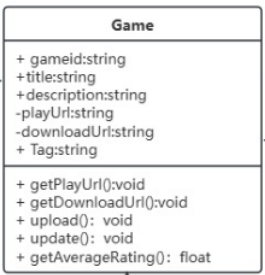
\includegraphics[width=0.4\textwidth]{./images/game.png} % 插入图片,设置宽度为页面宽度的 50%
      \caption{game类图} % 添加标题
  \end{figure}

  \begin{table}[H]
  \centering  % 居中表格
  \begin{tabular}{|c|c|}
    \hline
    测试内容 & 测试结果 \\
    \hline
    getPlayUrl& 通过 \\
    \hline
    getDownloadUrl& 通过 \\
    \hline
    upload& 通过 \\
    \hline
    update& 通过 \\
    \hline
    getAvarageRating& 通过 \\
    \hline
  \end{tabular}
\end{table}

\subsubsection{tag类}
  \begin{figure}[H] % 使用 figure 环境来插入图片
      \centering % 图片居中
      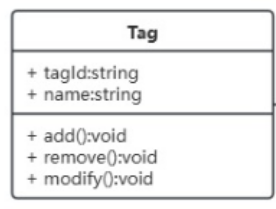
\includegraphics[width=0.4\textwidth]{./images/tag.png} % 插入图片,设置宽度为页面宽度的 50%
      \caption{tag类图} % 添加标题
  \end{figure}

  \begin{table}[H]
  \centering  % 居中表格
  \begin{tabular}{|c|c|}
    \hline
    测试内容 & 测试结果 \\
    \hline
    add& 通过 \\
    \hline
    remove& 通过 \\
    \hline
    modify& 通过 \\
    \hline
  \end{tabular}
\end{table}

\subsubsection{rating类}
  \begin{figure}[H] % 使用 figure 环境来插入图片
      \centering % 图片居中
      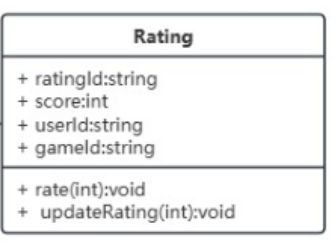
\includegraphics[width=0.4\textwidth]{./images/rating.png} % 插入图片,设置宽度为页面宽度的 50%
      \caption{rating类图} % 添加标题
  \end{figure}

  \begin{table}[H]
  \centering  % 居中表格
  \begin{tabular}{|c|c|}
    \hline
    测试内容 & 测试结果 \\
    \hline
    rate& 未通过 \\
    \hline
    updateRating& 未通过 \\
    \hline
  \end{tabular}
\end{table}

\subsubsection{tourist类}
\begin{figure}[H]
  \centering
  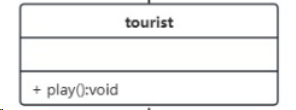
\includegraphics[width=0.4\textwidth]{tourist.png}
  \caption{tourist类图} % 添加标题
\end{figure}
\begin{table}[H]
  \centering
  \begin{tabular}{|ll|}
    \hline
    测试内容 & 测试结果 \\
    \hline
    play& 通过 \\
    \hline
  \end{tabular}
\end{table}


\subsubsection{user类}
\begin{figure}[H]
  \centering
  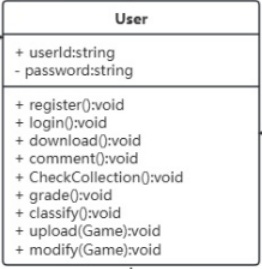
\includegraphics[width=0.4\textwidth]{user.png}
  \caption{user类图} % 添加标题
\end{figure}

  \begin{table}[H]
  \centering  % 居中表格
  \begin{tabular}{|c|c|}
    \hline
    测试内容 & 测试结果 \\
    \hline
    register& 通过 \\
    \hline
    login& 未通过 \\
    \hline
    download& 通过 \\
    \hline
    comment& 未通过 \\
    \hline
    CheckCollection& 未通过 \\
    \hline
    grade& 未通过 \\
    \hline
    classify& 通过 \\
    \hline
    upload& 通过 \\
    \hline
    modify& 通过 \\
    \hline
  \end{tabular}
\end{table}

\subsubsection{collection类}
\begin{figure}[H]
  \centering
  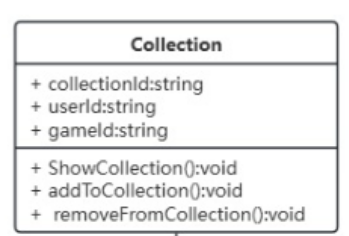
\includegraphics[width=0.4\textwidth]{collection.png}
  \caption{collection类图} % 添加标题
\end{figure}
  \begin{table}[H]
  \centering  % 居中表格
  \begin{tabular}{|c|c|}
    \hline
    测试内容 & 测试结果 \\
    \hline
    showCollection& 通过 \\
    \hline
    addToCollection& 通过 \\
    \hline
    removeFromCollection& 通过 \\
    \hline
  \end{tabular}
\end{table}

\subsubsection{comment类}
\begin{figure}[H]
  \centering
  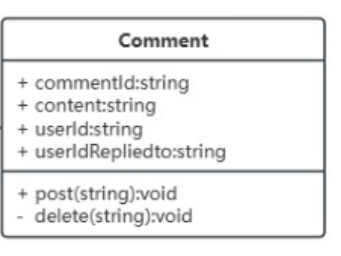
\includegraphics[width=0.4\textwidth]{comment.png}
  \caption{comment类图} % 添加标题
\end{figure}

  \begin{table}[H]
  \centering  % 居中表格
  \begin{tabular}{|c|c|}
    \hline
    测试内容 & 测试结果 \\
    \hline
    post& 未通过 \\
    \hline
    delete& 未通过 \\
    \hline
  \end{tabular}
\end{table}
\subsubsection{manager类}


\begin{figure}[H]
  \centering
  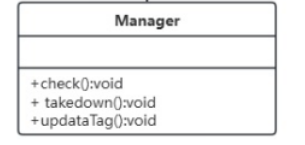
\includegraphics[width=0.4\textwidth]{manager.png}
  \caption{manager类图} % 添加标题
\end{figure}

  \begin{table}[H]
  \centering  % 居中表格
  \begin{tabular}{|c|c|}
    \hline
    测试内容 & 测试结果 \\
    \hline
    check & 通过 \\
    \hline
    takedown & 通过 \\
    \hline
    updateTag & 通过 \\
    \hline
  \end{tabular}
\end{table}

\subsubsection{Notification类}
\begin{figure}[H]
  \centering
  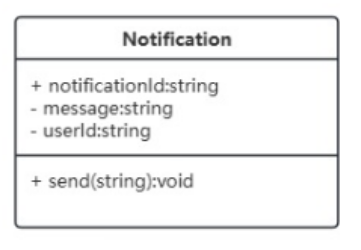
\includegraphics[width=0.4\textwidth]{notification.png}
  \caption{Notification类图} % 添加标题
\end{figure}

\begin{table}[H]
  \centering  % 居中表格
  \begin{tabular}{|c|c|}
    \hline
    测试内容 & 测试结果 \\
    \hline
    send & 未通过 \\
    \hline
  \end{tabular}
\end{table}

\subsection{类模型一致性测试}
为了确保类与类之间也可以正常合作,还需要对所有类的 CRC 模型进行测试。下面分别列出来针对每一个类的 CRC 模型和对应需要测试的项目。

game类:重点检查标签、下载和访问的链接是否能够正常使用。
\begin{table}[H]
  \centering
  \begin{tabular}{|ll|}  % 移除列间竖线
    \cline{1-2}  % 横跨两列的横线
    类名:& \textbf{game} \\
    \cline{1-2}
    描述:& 游戏本体。 \\
    \cline{1-2}
    \multicolumn{1}{|l|}{\textbf{功能}} &{\textbf{合作类}} \\  % 手动添加竖线
    \hline
    \multicolumn{1}{|l|}{getPlayUrl} &  \\
    \hline
    \multicolumn{1}{|l|}{getDownloadUrl} &  \\
    \hline
    \multicolumn{1}{|l|}{upload} &  \\
    \hline
    \multicolumn{1}{|l|}{update} &  \\
    \hline
    \multicolumn{1}{|l|}{getAvarageRating} & rating类 \\
    \hline
  \end{tabular}
\end{table}

tag类:检查标签的添加、删除和修改是否能够正常使用。
\begin{table}[H]
  \centering
  \begin{tabular}{|ll|}  % 移除列间竖线
    \cline{1-2}  % 横跨两列的横线
    类名:& \textbf{tag} \\
    \cline{1-2}
    描述:& 游戏标签。 \\
    \cline{1-2}
    \multicolumn{1}{|l|}{\textbf{功能}} & {\textbf{合作类}} \\  % 手动添加竖线
    \hline
    \multicolumn{1}{|l|}{add} &  \\
    \hline
    \multicolumn{1}{|l|}{remove} &  \\
    \hline
    \multicolumn{1}{|l|}{modify} &  \\
    \hline
  \end{tabular}
\end{table}

rating类:检查评分的添加和修改是否能够正常使用。
\begin{table}[H]
  \centering
  \begin{tabular}{|ll|}  % 移除列间竖线
    \cline{1-2}  % 横跨两列的横线
    类名:& \textbf{rating} \\
    \cline{1-2}
    描述:& 游戏评分。 \\
    \cline{1-2}
    \multicolumn{1}{|l|}{\textbf{功能}} & {\textbf{合作类}} \\  % 手动添加竖线
    \hline
    \multicolumn{1}{|l|}{rate} &  \\
    \hline
    \multicolumn{1}{|l|}{updateRating} &  \\
    \hline
  \end{tabular}
\end{table}

tourist类:检查游客的在线游玩功能是否能够正常使用,是否能够访问到game类信息。

\begin{table}[H]
  \centering
  \begin{tabular}{|ll|}  % 移除列间竖线
    \cline{1-2}  % 横跨两列的横线
    类名:& \textbf{tourist} \\
    \cline{1-2}
    描述:& 游客。 \\
    \cline{1-2}
    \multicolumn{1}{|l|}{\textbf{功能}} & {\textbf{合作类}} \\  % 手动添加竖线
    \hline
    \multicolumn{1}{|l|}{play} & {game类} \\
    \hline
  \end{tabular}
\end{table}

user类:检查用户的注册、登录、下载、评论、收藏、评分、分类、上传和修改功能是否能够正常使用。

\begin{table}[H]
  \centering
  \begin{tabular}{|ll|}  % 移除列间竖线
    \cline{1-2}  % 横跨两列的横线
    类名:& \textbf{user} \\
    \cline{1-2}
    描述:& 用户,继承自\textbf{user}。 \\
    \cline{1-2}
    \multicolumn{1}{|l|}{\textbf{功能}} &{\textbf{合作类}} \\  % 手动添加竖线
    \hline
    \multicolumn{1}{|l|}{register} & \\
    \hline
    \multicolumn{1}{|l|}{login} &  \\
    \hline
    \multicolumn{1}{|l|}{download} & {game类} \\
    \hline
    \multicolumn{1}{|l|}{comment} & {comment类} \\
    \hline
    \multicolumn{1}{|l|}{CheckCollection} & {collection类} \\
    \hline
    \multicolumn{1}{|l|}{grade} & {rating类、game类} \\
    \hline
    \multicolumn{1}{|l|}{classify} & {tag类、game类} \\
    \hline
    \multicolumn{1}{|l|}{upload} & {game类} \\
    \hline
    \multicolumn{1}{|l|}{modify} & {game类} \\
    \hline
  \end{tabular}
\end{table}

collection类:检查收藏的显示、添加和删除功能是否能够正常使用。
\begin{table}[H]
  \centering
  \begin{tabular}{|ll|}  % 移除列间竖线
    \cline{1-2}  % 横跨两列的横线
    类名:& \textbf{collection} \\
    \cline{1-2}
    描述:& 收藏。 \\
    \cline{1-2}
    \multicolumn{1}{|l|}{\textbf{功能}} & {\textbf{合作类}} \\  % 手动添加竖线
    \hline
    \multicolumn{1}{|l|}{showCollection} & {collection类}  \\
    \hline
    \multicolumn{1}{|l|}{addToCollection} & {game类、user类} \\
    \hline
    \multicolumn{1}{|l|}{removeFromCollection} & {game类、user类} \\
    \hline
  \end{tabular}
\end{table}

comment类:检查评论的发布和删除功能是否能够正常使用。
\begin{table}[H]
  \centering
  \begin{tabular}{|ll|}  % 移除列间竖线
    \cline{1-2}  % 横跨两列的横线
    类名:& \textbf{comment} \\
    \cline{1-2}
    描述:& 评论。 \\
    \cline{1-2}
    \multicolumn{1}{|l|}{\textbf{功能}} & {\textbf{合作类}} \\  % 手动添加竖线
    \hline
    \multicolumn{1}{|l|}{post} & {game类、user类} \\
    \hline
    \multicolumn{1}{|l|}{delete} & {game类、user类 }\\
    \hline
  \end{tabular}
\end{table}

manager类:检查管理员的检查、下架和更新标签功能是否能够正常使用。
\begin{table}[H]
  \centering
  \begin{tabular}{|ll|}  % 移除列间竖线
    \cline{1-2}  % 横跨两列的横线
    类名:& \textbf{manager} \\
    \cline{1-2}
    描述:& 管理员,继承自\textbf{user}。 \\
    \cline{1-2}
    \multicolumn{1}{|l|}{\textbf{功能}} & \multicolumn{1}{|l|}{\textbf{合作类}} \\  
    \hline
    \multicolumn{1}{|l|}{check} & \multicolumn{1}{|l|}{game类} \\
    \hline
    \multicolumn{1}{|l|}{takedown} & \multicolumn{1}{|l|}{game类} \\
    \hline
    \multicolumn{1}{|l|}{updateTag} & \multicolumn{1}{|l|}{tag类} \\
    \hline
  \end{tabular}
\end{table}

\section{功能验证测试}

\subsection{登录注册模块}
\begin{table}[H]
\centering
\begin{tabular}{|c|c|c|c|}
  \hline
  功能名称 & 输入 & 预期输出 & 实际输出 \\
  \hline
  登录 & 正确的用户名和密码 & 登录成功 & 与预期相符 \\
  \hline
  登录 & 错误的用户名和密码 & 登录失败 & 与预期相符 \\
  \hline
  注册 & 管理员导入用户信息 & 注册成功并生成随机密码 & 与预期相符 \\
  \hline
  \end{tabular}
\end{table}


\subsection{游戏上传模块}

\begin{table}[H]
  \centering
  \begin{tabular}{|c|c|c|c|}
    \hline
    功能名称 & 输入 & 预期输出 & 实际输出 \\
    \hline
    上传游戏 & 正确的游戏信息 & 上传成功 & 与预期相符 \\
    \hline
    上传游戏 & 错误的游戏信息 & 上传失败 & 与预期相符 \\
    \hline
    上传游戏 & 缺少必要信息 & 上传失败 & 与预期相符 \\
    \hline
  \end{tabular}
\end{table}

\subsection{游戏管理模块}

\begin{table}[H]
  \centering
  \begin{tabular}{|c|c|c|c|}
    \hline
    功能名称 & 输入 & 预期输出 & 实际输出 \\
    \hline
    删除游戏 & 正确的游戏ID & 删除成功 & 与预期相符 \\
    \hline
    删除游戏 & 错误的游戏ID & 删除失败 & 与预期相符 \\
    \hline
    修改游戏信息 & 正确的游戏ID和信息 & 修改成功 & 与预期相符 \\
    \hline
    修改游戏信息 & 错误的游戏ID和信息 & 修改失败 & 与预期相符 \\
    \hline
    修改游戏信息 & 缺少游戏ID & 修改失败 & 与预期相符 \\
    \hline
    审核游戏通过 & 正确的游戏ID & 审核成功 & 与预期相符 \\
    \hline
    审核游戏通过 & 错误的游戏ID & 审核失败 & 与预期相符 \\
    \hline
  \end{tabular}
\end{table}

\section{边界测试}
本小节主要针对各项功能的边界输入进行测试,以便确保系统的鲁棒性。 
\subsection{游戏管理模块}

\begin{table}[H]
\centering
\renewcommand{\arraystretch}{1.5} 
\begin{tabular}{|>{\centering\arraybackslash}p{2cm}|>{\raggedright\arraybackslash}p{5cm}|>{\raggedright\arraybackslash}p{5cm}|>{\raggedright\arraybackslash}p{4cm}|}
\hline
\textbf{功能名称} & \textbf{输入} & \textbf{预期输出} & \textbf{实际输出} \\
\hline
上传游戏 & 上传数据不合规的游戏上传表单 & 显示出操作失败的提示信息 & 与预期输出相符 \\
\hline
上传游戏 & 游客请求 & 显示无权限的提示信息 & 与预期输出相符 \\
\hline
更新游戏 & 上传数据不合规的游戏更新表单 & 显示出操作失败的提示信息 & 与预期输出相符 \\
\hline
查找游戏 & 输入不存在的游戏id/名称 & 显示出没有找到游戏的提示信息 & 与预期输出相符 \\
\hline
查找游戏 & 输入为空 & 显示出不能为空的提示信息 & 与预期输出相符 \\
\hline
下载游戏 & 游客请求下载 & 显示无权限的提示信息 & 与预期输出相符 \\
\hline
游玩游戏 & 游客请求私有游戏 & 显示无权限的提示信息 & 与预期输出相符 \\
\hline
\end{tabular}
\end{table}

\begin{table}[H]
\centering
\begin{tabular}{|c|c|c|c|}
  \hline
  功能名称 & 输入 & 预期输出 & 实际输出 \\
  \hline
  登录 & 错误的用户名和密码 & 登录失败 & 与预期相符 \\
  \hline
  登录 & 信息空缺 & 在登录界面出现错误提示 & 与预期相符 \\
  \hline
  \end{tabular}
\end{table}

\subsection{游戏上传模块}

\begin{table}[H]
  \centering
  \begin{tabular}{|c|c|c|c|}
    \hline
    功能名称 & 输入 & 预期输出 & 实际输出 \\
    \hline
    上传游戏 & 错误的游戏信息 & 上传失败 & 与预期相符 \\
    \hline
    上传游戏 & 文件容量过大 & 上传失败 & 与预期相符 \\
    \hline
    上传游戏 & 文件格式错误 & 上传失败 & 与预期相符 \\
    \hline
    上传游戏 & 传输过程断网 & 上传失败 & 与预期相符 \\
    \hline
    上传游戏 & 缺少必要信息 & 上传失败 & 与预期相符 \\
    \hline
  \end{tabular}
\end{table}

\subsection{游戏管理模块}

\begin{table}[H]
  \centering
  \begin{tabular}{|c|c|c|c|}
    \hline
    功能名称 & 输入 & 预期输出 & 实际输出 \\
    \hline
    删除游戏 & 空 & 删除失败 & 与预期相符 \\
    \hline
    删除游戏 & 错误的游戏ID & 删除失败 & 与预期相符 \\
    \hline
    修改游戏信息 & 错误的游戏ID和信息 & 修改失败 & 与预期相符 \\
    \hline
    修改游戏信息 & 缺少游戏ID & 修改失败 & 与预期相符 \\
    \hline
    审核游戏通过 & 错误的游戏ID & 审核失败 & 与预期相符 \\
    \hline
  \end{tabular}
\end{table}

\section{压力测试}
下面是当服务端处于高负载运行的情况下做出的测试。

\begin{table}[H]
\centering
\renewcommand{\arraystretch}{1.5} 

\begin{tabular}{|>{\centering\arraybackslash}p{4cm}|>{\raggedright\arraybackslash}p{5cm}|>{\raggedright\arraybackslash}p{5cm}|}
\hline
\textbf{功能名称} & \textbf{输入} & \textbf{输出} \\
\hline
登录 & 正常登录 & 系统运行正常 \\
\hline
个人信息更新 & 正常登录 & 系统运行正常 \\
\hline
查找用户 & 正常查找 & 系统运行正常 \\
\hline
查看用户信息 & 正常查看 & 系统运行正常 \\
\hline
获取首页游戏列表 & 正常查看 & 系统运行正常 \\
\hline
查找游戏 & 正常查找 & 系统运行正常 \\
\hline
游戏上传 & 正常上传 & 系统运行不正常 \\
\hline
游戏更新 & 正常更新 & 系统运行不正常 \\
\hline
\end{tabular}
\end{table}

\section{APIFox 接口测试}

我们使用 APIFox 方便地定义数据模型、接口文档、API 请求和 Mock 数据,
详细的接口文档可以在 APIFox 中查看,我们以不同权级角色对 API 接口进行分类,以下是一些重要的接口测试结果。

\subsection{游客相关接口}
\begin{table}[H]
\centering
\renewcommand{\arraystretch}{1.5} 
\begin{tabular}{|>{\centering\arraybackslash}p{2cm}|>{\raggedright\arraybackslash}p{3cm}|>{\raggedright\arraybackslash}p{4.5cm}|>{\raggedright\arraybackslash}p{5cm}|}
\hline
\textbf{接口名称} & \textbf{输入} & \textbf{预期输出} & \textbf{实际输出} \\
\hline
查看游戏列表 & 查看请求 & 返回游戏列表 & 与预期输出相符 \\
\hline
查找用户 & 用户id & 返回查找结果 & 与预期输出相符 \\
\hline
查看用户信息 & 用户id & 返回用户信息 & 与预期输出相符 \\
\hline
游玩公开游戏 & 游戏id & 返回游戏入口链接 & 与预期输出相符 \\
\hline
\end{tabular}
\end{table}

\subsection{开发者相关接口}
在游客的基础上,开发者可以拥有更多的权限。
\begin{table}[H]
\centering
\renewcommand{\arraystretch}{1.5} 
\begin{tabular}{|>{\centering\arraybackslash}p{2cm}|>{\raggedright\arraybackslash}p{3cm}|>{\raggedright\arraybackslash}p{4.5cm}|>{\raggedright\arraybackslash}p{5cm}|}
\hline
\textbf{接口名称} & \textbf{输入} & \textbf{预期输出} & \textbf{实际输出} \\
\hline
登录 & qq,密码 & 返回用户id,权限token & 与预期输出相符 \\
\hline
查看个人信息 & 查看请求 & 返回用户信息 & 与预期输出相符 \\
\hline
个人信息更新 & 更新信息 & 返回更新结果 & 与预期输出相符 \\
\hline
上传游戏 & 上传表单信息 & 返回上传结果 & 与预期输出相符 \\
\hline
更新游戏 & 更新表单信息 & 返回更新结果 & 与预期输出相符 \\
\hline
下载游戏 & 游戏id & 返回游戏文件 & 与预期输出相符 \\
\hline
\end{tabular}
\end{table}

\subsection{管理员相关接口}
\begin{table}[H]
\centering
\renewcommand{\arraystretch}{1.5} 
\begin{tabular}{|>{\centering\arraybackslash}p{2cm}|>{\raggedright\arraybackslash}p{3cm}|>{\raggedright\arraybackslash}p{4.5cm}|>{\raggedright\arraybackslash}p{5cm}|}
\hline
\textbf{接口名称} & \textbf{输入} & \textbf{预期输出} & \textbf{实际输出} \\
\hline
删除游戏 & 游戏id & 返回删除结果 & 与预期输出相符 \\
\hline
审核游戏 & 审核结果 & 返回提交结果 & 与预期输出相符 \\
\hline
删除用户 & 用户id & 返回删除结果 & 与预期输出相符 \\
\hline
批量创建用户 & qq,用户名 & 返回创建结果 & 与预期输出相符 \\
\hline
换绑用户qq & id,qq & 返回更新结果 & 与预期输出相符 \\
\hline
\end{tabular}
\end{table}

\section{网页性能测试}
网页的性能是影响用户体验的重要因素之一,这包括了网页的加载速度,响应速度,内存使用等。
下面将使用开发者工具中的性能测试功能对网页进行测试。


\subsection{错误页保护}

在用户访问不存在的页面时,网页会自动跳转到错误页,提示用户该页面不存在。
\begin{figure}[H]
  \centering
  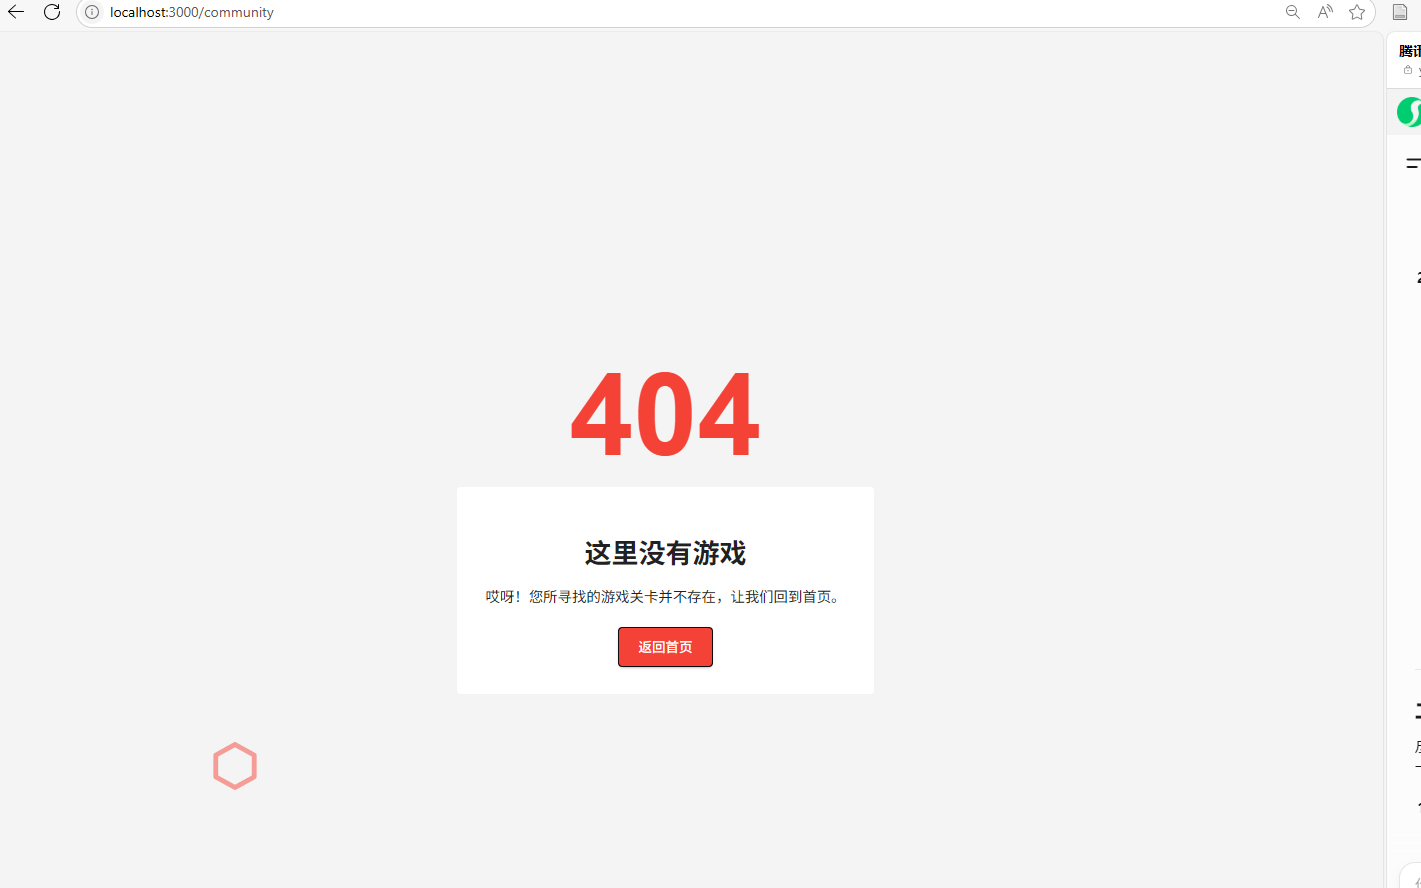
\includegraphics[width=0.8\textwidth]{front-page3.png}
  \caption{错误页}
\end{figure}

而在网络延迟较高,例如下方网络延迟测试中的 4.5s 白屏时间,用户界面会显示加载中,提示用户页面仍然在加载,起到提升用户体验的方式。


\begin{figure}[H]
  \centering
  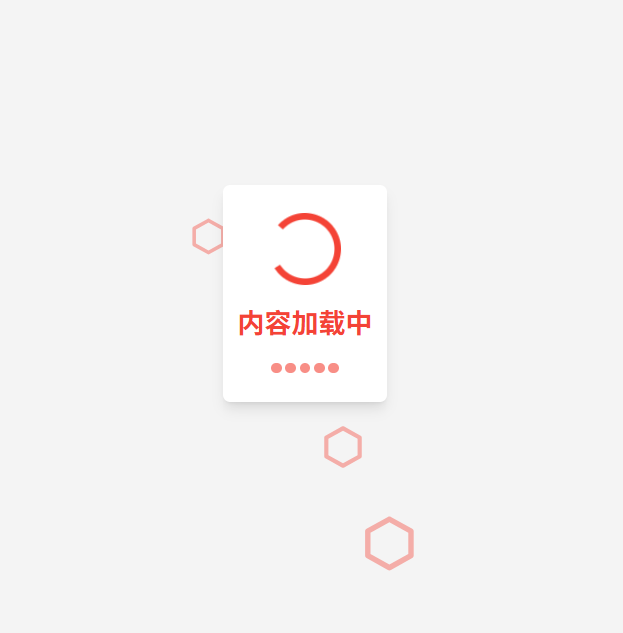
\includegraphics[width=0.8\textwidth]{front-page5.png}
  \caption{加载页}
\end{figure}

\subsection{网络延迟}

开启网络中的 “禁用缓存”,以反映真实的网络延迟。首先压力测试慢速 3D 网络环境下网页的表现和加载速度。

可以发现,由于使用 Next.js 框架,网页不会出现布局抖动的问题,大部分文字快速加载出来,
而图片使用了懒加载的方式,只有在用户滚动到图片位置时才会加载图片。
而由于所有的 JPEG 图片都使用 基线 加载格式,因此在慢速网络环境下会加载出上半部分。

\begin{figure}[H]
  \centering
  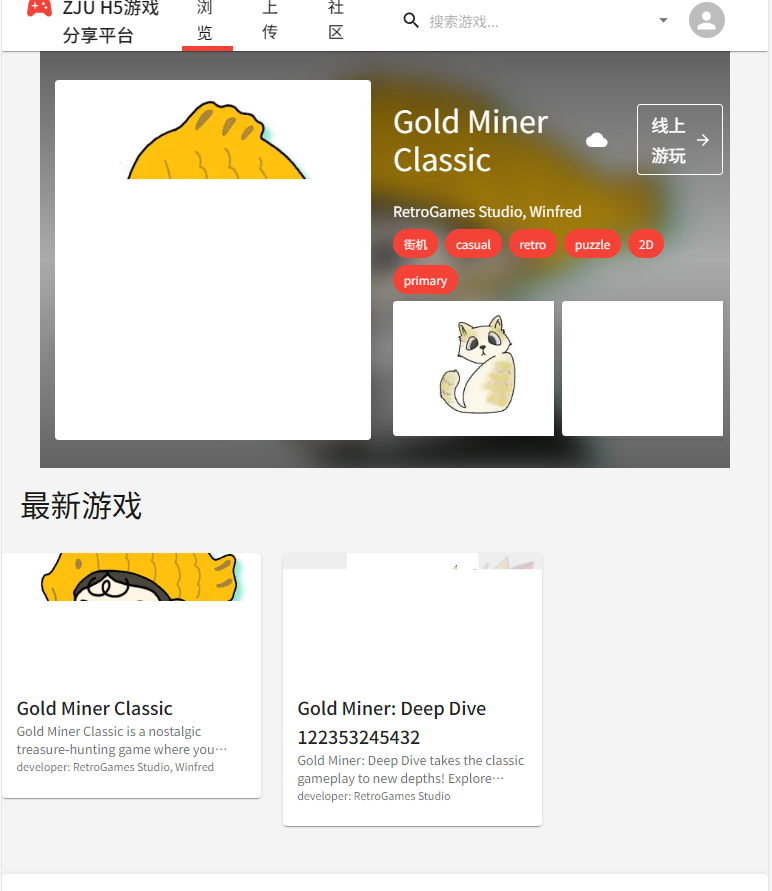
\includegraphics[width=0.8\textwidth]{front-page1.png}
  \caption{慢速 3G 加载测试 - 网页图}
\end{figure}

排除开发环境下 HMR 热更新请求带来的额外开销,从下图可见,整体网页在 4.5s 左右就已经加载好所有样式和文字内容(白线处),反映出较好的白屏等待时间
;而图片的加载速度由于过慢,完成时间在 30s 左右,这在慢速网络中是合理的。

\begin{figure}[H]
  \centering
  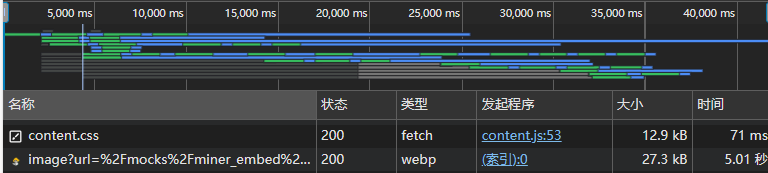
\includegraphics[width=0.8\textwidth]{front-page2.png}
  \caption{慢速 3G 加载测试 - 时间轴}
\end{figure}

\subsection{内存使用}
由于 js 自带有 GC 垃圾回收机制,因此内存使用的情况并不明显,我们挑选内存消耗最大的游戏游玩界面,因为嵌入 iframe 而要求较高的内存使用。
可以发现,总体使用内存在 80MB 左右,并没有达到浏览器的限制,且在游玩游戏时内存使用并没有明显增加。因此在内存使用上表现良好。
\begin{figure}[H]
  \centering
  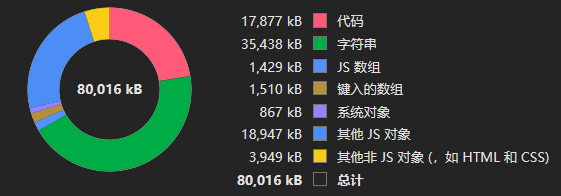
\includegraphics[width=0.8\textwidth]{front-page4.png}
  \caption{内存使用环形图}
\end{figure}

\section{对软件功能的结论}

\subsection{游戏管理模块}
该模块实现了增删改游戏,以及游戏查找,下载,游玩的功能。 
经过测试,功能正常,在性能上具有一定的稳定性和鲁棒性,
但在处理游戏大文件时存在处理慢,并发性差的问题,与用户交互界面友好。
\subsection{普通用户模块}
该模块实现了游客与开发者对自身的一些操作,如登录,个人信息的查看与更新,用户的查找,
以及对游戏的收藏,查看,下载,游玩等功能。
经过测试,功能正常,在性能上具有一定的稳定性和鲁棒性,
与用户交互界面良好。
\subsection{管理员模块}
该模块实现了管理员的一系列操作,包括用户的删除,批量创建,
游戏的删除,审核,换绑qq等功能。
经过测试,功能正常,在性能上具有一定的稳定性和鲁棒性,
与用户交互界面良好。
\section{分析总结}
\subsection{能力}
经过上述面向对象测试、功能测试、边界测试、压力测试和APIFOX接口测试,本系统的
大部分预定功能都已经得到了正确的实现,并且能够应对各种边界输入,具有一定的稳定行
和鲁棒性,也基本达到了用户需求。
\subsection{限制}
本系统在应对高并发方面的能力有限,
在响应速度与处理速度方面的能力有限,
并且在功能上还有许多可拓展空间,比如在游戏的评论区功能,
游戏的评分功能等。一些已经实现的功能也存在优化空间。
\end{document}